\section{Программное обеспечение системы}

% \subsection{Структура программного обеспечения и функции его компонентов}
% Work in process.

\subsection{Выбор компонентов программного обеспечения}

\subsubsection{Инструментальное средство разработки и язык программирования}

На данный момент существует огромное множество языков программирования, на которых можно разработать веб-ориентированную информационную систему.

Для выбора необходимого языка программирования была составлена сравнительная характеристика трёх самых распространённых и динамично развивающихся языков, используемых в сети Интернет~\cite{chikagosHub,leonardTeo}.
Результаты анализа приведены в таблице~\ref{tab:software-language}.

\begin{footnotesize}
\begin{longtable}[h]{|p{0.3\textwidth}|p{0.2\textwidth}|p{0.2\textwidth}|p{0.2\textwidth}|}
	\caption{\label{tab:software-language}Сравнительных анализ языков программирования веб-ориентированных ИС} \\
	\hline
		\textbf{Критерий} &
		\textbf{PHP} &
		\textbf{Ruby} &
		\textbf{C\#} \\
	\hline \endfirsthead
	\hline
		\textbf{Критерий} &
		\textbf{PHP} &
		\textbf{Ruby} &
		\textbf{C\#} \\
	\hline \endhead
	Скорость формирования страницы & 
	средне & медленно & быстро \\ \hline
	
	Нагрузка пользователей & 
	мало & мало & много \\ \hline
	
	Лёгкость и скорость разработки & 
	легко & очень легко & средне \\ \hline
	
	Наличие фреймворков & 
	есть & есть & есть \\ \hline
	
	Расширенная обработка исключений & 
	нет	& есть & есть \\ \hline
	
	Сложность генерации отчётов & 
	высокая & высокая & низкая \\ \hline
\end{longtable}
\end{footnotesize}

Сложность генерации отчётов включает сложность создания и отображения отчёта, предоставляемого пользователю.

Ввиду того, что информационная система будет открытой для гостей, необходимо иметь высокую скорость формирования динамических страниц.
Также в техническом задании указано наличие расширенной обработки исключений и отклика отчётных форм.
На основании данных критериев, а также используемого языка при написании регионального сегмента ГИС ЖКХ, был выбран язык программирования C\# и, соответственно, платформа .NET.

Для данного языка программирования существует несколько программных\linebreak средств: разрабатываемая корпорацией Microsoft среда разработки Visual Studio, свободная среда разработки Xamarin Studio, а также другие менее функциональные аналоги.
Сравнительный анализ Visual Studio и Xamarin Studio представлен в таблице~\ref{tab:software-sharpide}.

\begin{footnotesize}
\begin{longtable}[h]{|p{0.5\textwidth}|p{0.2\textwidth}|p{0.2\textwidth}|}
	\caption{\label{tab:software-sharpide}Сравнительный анализ средств разработки на C\#} \\
	\hline
		\textbf{Критерий} &
		\textbf{Visual Studio} &
		\textbf{Xamarin} \\
	\hline \endfirsthead
	\hline
		\textbf{Критерий} &
		\textbf{Visual Studio} &
		\textbf{Xamarin} \\
	\hline \endhead
	Подсветка синтаксиса & 
	есть & есть \\ \hline
	
	Дизайнер веб-форм & 
	есть & нет \\ \hline
	
	Дизайнер модели данных & 
	есть & нет \\ \hline
	
	Кроссплатформенность & 
	нет & есть \\ \hline
	
	Интеграция с CVS & 
	есть & есть \\ \hline
\end{longtable}
\end{footnotesize}

Как можно видеть из представленного анализа, оба инструментальных средства имеют преимущества друг перед другом.
Но так как дизайнер модели данных и веб-форм важнее кроссплатформенности (для разработки можно установить и виртуальную машину с необходимой ОС), то для разработки было принято решение использовать Microsoft Visual Studio.

Согласно спецификации Microsoft, для поддержки .NET framework 4 и 4.5 (требуется техническим заданием) необходима Microsoft Visual Studio, начиная с версии 2012~\cite{vs_mdn}.
Была выбрана версия 2013 ввиду увеличения удобства пользования, в сравнении с предыдущей версией среды разработки.

\subsubsection{Операционная система}

Ввиду того, что информационная система является веб-ориентированной, то для запуска клиентской части необходима любая операционная система, поддерживающая приложения-браузеры.

Для выбора операционной системы, на которой будет выполняться серверная часть, рассмотрим две современные операционные системы, широко использованные для размещения веб-серверов: Microsoft Windows и GNU/Linux~\cite{sunHosting}.

Как известно, обе операционные системы отлично справляются с высокими нагрузками пользователей, имеют большое количество прикладного программного обеспечения, полную и понятную документацию.
Также обе операционные системы имеют собственные реализации стека сетевых протоколов модели OSI, что вносит некоторое разнообразие в механизм обработки запроса от клиентов.
Но, в любом случае, эти различия не сильно сказываются на производительности веб-сервера.
Основную роль в выборе операционной системы сыграл пункт 1.5.3 технического задания, по которому система должна корректно запускаться и функционировать на ОС Windows Server 2008 R2.

В дополнение к выбору именно этой операционной системы можно отметить, что существует отличие в наборе инструментария для администрирования и размещения веб-проектов на основе технологий .NET.
В Microsoft Windows эти инструментарии легко подключаются и настраиваются.
В GNU/Linux также присутствуют свободные аналоги, но они не претендуют на полноту и огромную практическую значимость.

Таким образом, для разворачивания серверной части информационной системы была выбрана ОС Microsoft Windows Server 2008 R2.

\subsubsection{Средство функционального моделирования}

При разработке программного проекта рекомендуемым процессом является описание бизнес-процессов, автоматизацию которых необходимо проводить.
Для этого следует использовать программное обеспечение, обеспечивающее функциональное моделирование.

Для описания процессов предметной области была выбрана диаграмма IDEF0.

Прикладных программ, реализующих разработку данной диаграммы, множество, но они либо скудны в функциональности, устарели или платные.

Была выбрана программа Ramus Educational, которая является бесплатным аналогом бывшей BPwin (сейчас AllFusion Process Modeller).
Данная программа поддерживает создание диаграмм IDEF0, DFD, а также работу с классификаторами.
При разработке выпускной квалификационной работы этого достаточно.
Помимо этого данная программа корректно запускается на современных версиях операционной системы Microsoft Windows в отличие от устаревшего BPwin.

\subsubsection{Средство информационного моделирования}

Разработка информационной модели также необходима, как и разработка функциональной модели. Для описания такой модели была выбрана диаграмма IDEF1X.

Для разработки информационной модели была выбрана программа ERwin 7, так как уже существует лицензия на её использование.
Аналогом данной программы является ER Constructor, разрабатываемый на кафедре ИВК УлГТУ.
Но огромным недостатком данного программного обеспечения является нелогичное рисование связей между сущностями при их перемещении.
Из недостатков Erwin 7 можно отметить отсутствие поддержки последних версий операционной системы Microsoft Windows (8, 8.1 и более новых), так как последняя версия программы вышла в 2007 году.
Это отсутствие ощущается при сворачивании-разворачивании окна с программой: при этих действиях иногда модель перестаёт перерисовывать, и это необходимо делать самостоятельно при помощи соответствующей команды в меню.

\subsubsection{Вспомогательное программное обеспечение}

В дополнение к изложенным выше инструментальным средствам, для разработки информационной системы было использовано следующее программное обеспечение:

\begin{easylist}
& система управления версиями. Выбор между GIT и SVN ввиду простоты последнего был сделан в пользу SVN;
& графический пакет. Был выбран GIMP в силу бесплатности и широких возможностей. Аналогами являются Adobe Photoshop и Paint.NET;
& веб-сервер. При развёртке проекта на C\#, доступны два веб-сервера: IIS и IIS Express. Ввиду того, что функциональность последнего вполне достаточна для разработки и отладки разрабатываемой системы, был выбран он;
& система учёта задач и ошибок. Был использован Redmine из-за того, что он уже на протяжении трёх лет используется у заказчика информационной системы. Аналогами являются Jira и Bugzilla.
\end{easylist}

\subsection{Разработка прикладного программного обеспечения}

\subsubsection{Структура прикладного программного обеспечения}

Система состоит из двух подсистем: <<АРМ подрядной организации>>, делимый на модули открытой части и личного кабинета, и <<АРМ РОКР>>, в котором можно выделить модули отбора подрядчиков, проведения конкурсов и учёта договоров капитального ремонта.
Данное дробление системы на подсистемы и модули было выбрано ввиду явного разделения функций системы согласно техническому заданию.

Спецификация подсистемы <<АРМ подрядной организации>> представлена в таблице~\ref{tab:software-specArmContractor}.

\begin{footnotesize}
\begin{longtable}[h]{|p{0.05\textwidth}|p{0.3\textwidth}|p{0.55\textwidth}|}
	\caption{\label{tab:software-specArmContractor}Спецификация подсистемы <<АРМ подрядной организации>>} \\
	\hline
		\thead{№} & \thead{Название компонента} & \thead{Описание} \\
	\hline
		\theadnum{1} & \theadnum{2} & \theadnum{3} \\
	\hline \endfirsthead
	\hline
		 \theadnum{1} & \theadnum{2} & \theadnum{3} \\
	\hline \endhead
	\multicolumn{3}{|c|}{\textbf{Модули}} \\ \hline
	1 & Open & Открытая часть портала, доступная любому пользователю. \\ \hline
	2 & Personal & Личный кабинет подрядной организации. \\ \hline
	\multicolumn{3}{|c|}{\textbf{Подключаемые компоненты}} \\ \hline
	1 & AIS.HM.Model & Модель данных ИС <<Объектовый учёт>>. \\ \hline
	2 & KendoUI & Библиотека графического интерфейса. Используется для отображение таблиц и фильтров. \\ \hline
\end{longtable}
\end{footnotesize}

Спецификация подсистемы <<АРМ РОКР>> представлена в таблице~\ref{tab:software-specArmOperator}.

\begin{footnotesize}
\begin{longtable}[h]{|p{0.05\textwidth}|p{0.3\textwidth}|p{0.55\textwidth}|}
	\caption{\label{tab:software-specArmOperator}Спецификация подсистемы <<АРМ РОКР>>} \\
	\hline
		\thead{№} & \thead{Название компонента} & \thead{Описание} \\
	\hline
		\theadnum{1} & \theadnum{2} & \theadnum{3} \\
	\hline \endfirsthead
	\hline
		 \theadnum{1} & \theadnum{2} & \theadnum{3} \\
	\hline \endhead
	\multicolumn{3}{|c|}{\textbf{Модули}} \\ \hline
	1 & ContractorRequest & Модуль отбора подрядчиков. \\ \hline
	2 & Contest & Модуль проведения конкурсов. \\ \hline
	2 & ContractOnWork & Модуль учёта договоров на капитальный ремонт. \\ \hline
	\multicolumn{3}{|c|}{\textbf{Подключаемые компоненты}} \\ \hline
	1 & AIS.HM.Model & Модель данных ИС <<Объектовый учёт>>. \\ \hline
\end{longtable}
\end{footnotesize}

\subsubsection{Программный модуль <<АРМ подрядной организации --- открытая часть>>}

Спецификация модуля указана в таблице~\ref{tab:software-specArmContractorOpen}.

\begin{footnotesize}
\begin{longtable}[h]{|p{0.05\textwidth}|p{0.45\textwidth}|p{0.4\textwidth}|}
	\caption{\label{tab:software-specArmContractorOpen}Спецификация модуля Open} \\
	\hline
		\thead{№} & \thead{Название и тип элемента} & \thead{Описание} \\
	\hline
		\theadnum{1} & \theadnum{2} & \theadnum{3} \\
	\hline \endfirsthead
	\hline
		 \theadnum{1} & \theadnum{2} & \theadnum{3} \\
	\hline \endhead
	\multicolumn{3}{|c|}{\textbf{Классы-контроллеры}} \\ \hline
	1 & public class AccountController & Содержит методы для авторизации и регистрации пользователей. \\ \hline
	2 & public class BidController & Содержит методы для добавления заявки на КР. \\ \hline
	3 & public class ContestController & Содержит методы для просмотра конкурсов. \\ \hline
	4 & public class ContractController & Содержит методы для просмотра договоров на КР. \\ \hline
	5 & public class CostEstimationController & Содержит методы для просмотра смет (планов работ). \\ \hline
	6 & public class HomeController & Содержит методы для отображения главных страниц и страниц с ошибкой. \\ \hline
	7 & public class LotController & Содержит методы для просмотра лотов. \\ \hline
	8 & public class OrganizationController & Содержит методы для просмотра информации о подрядчике. \\ \hline
	9 & public class PortfolioController & Содержит методы для просмотра портфолио подрядчика. \\ \hline
	10 & public class StatsController & Содержит методы формирования статистики. \\ \hline
	\multicolumn{3}{|c|}{\textbf{Классы для авторизации}} \\ \hline
	1 & public class CheckFieldResult & Предоставляет результат заполнения полей при регистрации. \\ \hline
	2 & public class LoginModel & Содержит список полей для страницы авторизации. \\ \hline
	3 & public class PasswordModel & Содержит список полей для смены пароля. \\ \hline
	4 & public class RegisterModel & Модель данных для первого этапа регистрации. \\ \hline
	5 & public class RegisterSpecificModel & Модель данных для второго этапа регистрации. \\ \hline
	6 & public sealed class UserPrincipal & Паспорт пользователя. \\ \hline
	7 & public partial class UserIdentity & Идентификатор пользователя. \\ \hline
	8 & public class AccountMembershipService & Сервис для авторизации и регистрации пользователя. \\ \hline
	9 & public class FormsAuthenticationService & Сервис для аутентификации. \\ \hline
	\multicolumn{3}{|c|}{\textbf{Классы для заявок}} \\ \hline
	1 & public class BidRepository & Доступ к данным для списка заявок. \\ \hline
	\multicolumn{3}{|c|}{\textbf{Классы для смет}} \\ \hline
	1 & public class LotCostEstimationElement & Элемент агрегированной сметы по лоту \\ \hline
	\multicolumn{3}{|c|}{\textbf{Классы для статистики}} \\ \hline
	1 & public class StatsDataItem & Элемент статистики \\ \hline
	2 & public class StatsHomeViewModel & Модель представления для статистики на главной странице. \\ \hline
\end{longtable}
\end{footnotesize}

Для каждого контроллера есть классы [имя]Filter, в котором содержатся поля для фильтрации записей, а также [имя]ViewModel, который представляет собой модель представления для страниц, формируемых при помощи соответствующего контроллера.

% Описание действий контроллеров:
% \begin{enumerate}
	% \item AccountController:
	% \begin{enumerate}
		% \item public ActionResult RegisterWelcome()
		% \item public ActionResult RegisterGeneral()
		% \item [HttpPost] public ActionResult RegisterGeneral(RegisterModel model)
		% \item public ActionResult RegisterSpecific()
		% \item [HttpPost] public ActionResult RegisterSpecific(RegisterSpecificModel model)
		% \item public ActionResult RegisterPortfolio()
		% \item public ActionResult RegisterSuccess()
		% \item [HttpPost] public ActionResult Login()
		% \item [HttpPost] public ActionResult Login(LoginModel model, string returnUrl)
	% \end{enumerate}
	% \item 2
	% \item 3
	% \item 4
% \end{enumerate}

\subsubsection{Программный модуль <<АРМ подрядной организации --- личный кабинет>>}

Спецификация модуля указана в таблице~\ref{tab:software-specArmContractorPersonal}.

\begin{footnotesize}
\begin{longtable}[h]{|p{0.05\textwidth}|p{0.45\textwidth}|p{0.4\textwidth}|}
	\caption{\label{tab:software-specArmContractorPersonal}Спецификация модуля Personal} \\
	\hline
		\thead{№} & \thead{Название и тип элемента} & \thead{Описание} \\
	\hline
		\theadnum{1} & \theadnum{2} & \theadnum{3} \\
	\hline \endfirsthead
	\hline
		 \theadnum{1} & \theadnum{2} & \theadnum{3} \\
	\hline \endhead
	\multicolumn{3}{|c|}{\textbf{Классы-контроллеры}} \\ \hline
	1 & public class AssociationController & Содержит методы для работы с СРО. \\ \hline
	2 & public class BidController & Содержит методы для просмотра собственных заявок. \\ \hline
	3 & public class ContractActualInfoController & Содержит методы для отчётности по работам капитального ремонта. \\ \hline
	4 & public class ContractController & Содержит методы для работы с договорами на КР. \\ \hline
	5 & public class EmployeeController & Содержит методы для учёта сотрудников. \\ \hline
	6 & public class OrganizationController & Содержит методы для работы с информацией о подрядчике. \\ \hline
	7 & public class PortfolioController & Содержит методы для работы с портфолио подрядчика. \\ \hline
	8 & public class UserController & Содержит методы для доступа пользователей подрядчика к системе. \\ \hline
	\multicolumn{3}{|c|}{\textbf{Классы для OrganizationController}} \\ \hline
	1 & public class FillInfo & Элемент шкалы заполненности информации на главной странице личного кабинета. \\ \hline
\end{longtable}
\end{footnotesize}

Для каждого контроллера есть классы [имя]Filter, в котором содержатся поля для фильтрации записей, а также [имя]ViewModel, который представляет собой модель представления для страниц, формируемых при помощи соответствующего контроллера.

\subsubsection{Программный модуль <<АРМ РОКР --- Отбор подрядчиков>>}

Спецификация программного модуля представлена на таблице~\ref{tab:software-specArmRokrContractorRequest}.

\begin{footnotesize}
\begin{longtable}[h]{|p{0.05\textwidth}|p{0.45\textwidth}|p{0.4\textwidth}|}
	\caption{\label{tab:software-specArmRokrContractorRequest}Спецификация модуля ContractorRequest} \\
	\hline
		\thead{№} & \thead{Название и тип элемента} & \thead{Описание} \\
	\hline
		\theadnum{1} & \theadnum{2} & \theadnum{3} \\
	\hline \endfirsthead
	\hline
		 \theadnum{1} & \theadnum{2} & \theadnum{3} \\
	\hline \endhead
	\multicolumn{3}{|c|}{\textbf{Классы-контроллеры}} \\ \hline
	1 & public class ContractorRequestController & Содержит методы для отбора подрядных организаций. \\ \hline
	\multicolumn{3}{|c|}{\textbf{Методы класса ContractorRequestController}} \\ \hline
	1 & public ActionResult ListForOperator (ContractorRequestFilterModel filter) & Отображает список заявок на одобрение для РОКР. \\ \hline
	2 & public ActionResult Edit (int? id, ContractorRequestFilterModel filter) & Отображает страницу одобрения заявки. \\ \hline
	3 & [HttpPost] public ActionResult Edit (int? id, ContractorRequestFilterModel filter, int? status) & Одобряет заявку подрядчика. \\ \hline
\end{longtable}
\end{footnotesize}

\subsubsection{Программный модуль <<АРМ РОКР --- Проведение конкурсов>>}

Спецификация программного модуля представлена на таблице~\ref{tab:software-specArmRokrContest}.

\begin{footnotesize}
\begin{longtable}[h]{|p{0.05\textwidth}|p{0.45\textwidth}|p{0.4\textwidth}|}
	\caption{\label{tab:software-specArmRokrContest}Спецификация модуля Contest} \\
	\hline
		\thead{№} & \thead{Название и тип элемента} & \thead{Описание} \\
	\hline
		\theadnum{1} & \theadnum{2} & \theadnum{3} \\
	\hline \endfirsthead
	\hline
		 \theadnum{1} & \theadnum{2} & \theadnum{3} \\
	\hline \endhead
	\multicolumn{3}{|c|}{\textbf{Классы-контроллеры}} \\ \hline
	1 & public class ContestController & Содержит методы для работы с конкурсами. \\ \hline
	2 & public class ContractorController & Содержит методы для работы с подрядчиками. \\ \hline
	3 & public class CostEstimationController & Содержит методы для работы с лотами и сметами. \\ \hline
	4 & public class BidController & Содержит методы для работы с заявками. \\ \hline
	% \multicolumn{3}{|c|}{\textbf{Методы класса ContractorRequestController}} \\ \hline
	% 1 & public ActionResult ListForOperator (ContractorRequestFilterModel filter) & Отображает список заявок на одобрение для РОКР. \\ \hline
	% 2 & public ActionResult Edit (int? id, ContractorRequestFilterModel filter) & Отображает страницу одобрения заявки. \\ \hline
	% 3 & [HttpPost] public ActionResult Edit (int? id, ContractorRequestFilterModel filter, int? status) & Одобряет заявку подрядчика. \\ \hline
\end{longtable}
\end{footnotesize}

\subsubsection{Программный модуль <<АРМ РОКР --- Учёт договоров на КР>>}

Спецификация программного модуля представлена на таблице~\ref{tab:software-specArmRokrContractOnWork}.

\begin{footnotesize}
\begin{longtable}[h]{|p{0.05\textwidth}|p{0.45\textwidth}|p{0.4\textwidth}|}
	\caption{\label{tab:software-specArmRokrContractOnWork}Спецификация модуля ContractOnWork} \\
	\hline
		\thead{№} & \thead{Название и тип элемента} & \thead{Описание} \\
	\hline
		\theadnum{1} & \theadnum{2} & \theadnum{3} \\
	\hline \endfirsthead
	\hline
		 \theadnum{1} & \theadnum{2} & \theadnum{3} \\
	\hline \endhead
	\multicolumn{3}{|c|}{\textbf{Классы-контроллеры}} \\ \hline
	1 & public class ContractOnWorkController & Содержит методы для работы с договорами на КР. \\ \hline
	\multicolumn{3}{|c|}{\textbf{Методы класса ContractOnWorkController}} \\ \hline
	1 & public ActionResult TotalLots (ContractOnWorkFiltrerModel filter) & Отображает список договоров на КР. \\ \hline
	2 & public ActionResult EditContractOnWork (ContractOnWorkFiltrerModel filter, int id, bool isEdit) & Изменяет договор на КР. \\ \hline
	4 & public ActionResult ContractHistoryList (ContractOnWorkFiltrerModel filter, int id) & Список истории состояний договора на КР. \\ \hline
	5 & public ActionResult ContractDetails (ContractOnWorkFiltrerModel filter, int id) & Подробности договора на КР. \\ \hline
	6 & public ActionResult ConfirmContractPlan (ContractOnWorkFiltrerModel filter, int id) & Подтвердить плановые показатели. \\ \hline
	8 & public ActionResult ConfirmContractFact (ContractOnWorkFiltrerModel filter, int id) & Подтвердить фактические показатели. \\ \hline
	10 & public ActionResult ContractWorkTypeList (ContractOnWorkFiltrerModel filter) & Список видов работ. \\ \hline
	11 & public ActionResult ContractWorkTypeEdit (ContractOnWorkFiltrerModel filter, int? id) & Изменение вида работ. \\ \hline
	13 & public ActionResult ContractWorkTypeDelete (ContractOnWorkFiltrerModel filter, int id) & Удаление вида работ. \\ \hline
	14 & public ActionResult ElementDetails (ContractOnWorkFiltrerModel filter, int id) & Подробности элемента договора на КР. \\ \hline
	15 & public ActionResult EditReportDocuments (ContractOnWorkFiltrerModel filter, int id) & Изменение отчётных документов по КР. \\ \hline
	16 & public ActionResult ChangeStatus (ContractOnWorkFiltrerModel filter, int id) & Смена статуса договора на КР. \\ \hline
	17 & public ActionResult EditElementPlan (ContractOnWorkFiltrerModel filter, int? id, int contractElementId, int ElementId) & Изменить элемент плановых показателей. \\ \hline
	18 & public ActionResult EditElementFact (ContractOnWorkFiltrerModel filter, int? id, int contractElementId, int ElementId) & Изменить элемент фактических показателей. \\ \hline
\end{longtable}
\end{footnotesize}

\subsection{Разработка инструментального средства тестирования}

Было разработано приложение на основе технологии SlimerJs для реализации тестирования графического интерфейса пользователя.

Язык программирования --- JavaScript.

В приложении реализована очередь ссылок, по которым программа должна зайти и сделать скриншот веб-страницы.
Затем сниски экрана сохраняются в отдельной директории, откуда пользователь может получить к ним доступ.

Исходные тексты приложения указаны в приложении В.

% \subsection{Особенности реализации, эксплуатации и сопровождения системы}
% Work in process.

\subsection{Интерфейс пользователя с системой}

\subsubsection{Модели и технологии взаимодействия пользователя с системой}

Взаимодействие с системой производится за счёт перехода пользователя по гиперссылкам, вводу текстовой информации, прикреплению файлов и нажатию на кнопки.

Для того, чтобы попасть в определённый раздел системы, необходимо выбрать его в меню слева как ИС <<Объектовый учёт>>, где располагается АРМ РОКР, так и в ИС <<Портал подрядных организаций>>, где находится АРМ подрядной организации.

При выборе определённой функциональности (например, работа с конкурсами на капитальный ремонт), обычно сперва открывается страница с табличными данными, выше которых обычно содержится блок фильтров.
Фильтры могут быть текстовыми (поле адреса, название конкурса), логическими (только конкурсы с активными лотами), списочными (заявки со статусом <<не расмотрена РОКР>>), датой (начала, окончания чего-либо) и промежутком (максимальная стоимость работ).

Чтобы просмотреть подробную информацию о каком-либо объекте, на странице с табличными данными необходимо либо перейти по ссылке в названии необходимого объекта, либо нажать на кнопку <<Подробнее>>, находящейся в первой ячейке строки.

Если доступны какие-то действия над объектом, они будут отображаться либо в первой ячейке строки с таблицей этих объектов, либо над его описанием на странице подробностей.

Текст ошибки выводится либо около поля ввода, где были введены некорректные данные, либо вверху страницы под её заголовком в красном блоке.

\subsection{Руководство пользователя}

\subsubsection{Требования к условиям эксплуатации}

Для эксплуатации приложения требуется современная программа-браузер, например, последняя версия Google Chrome или Mozilla Firefox.
Требования к аппаратному обеспечению следует рассчитывать из требований браузера.

Для использования системы можно использовать компьютеры фирмы Apple со встроенным в операционную системы Mac OS X браузером Safari.
Система корректно отображает изображения меню на retina-дисплеях.

От пользователей системы требуется опыт работы с браузерами, а именно они должны знать как переходить по ссылкам, вводить данные в поля ввода.
Пользователи системы должны интуитивно воспринимать области нажатия страницы (то есть те места, куда можно нажать мышью или пальцем, чтобы произошло какое-либо действие).

\subsubsection{Порядок и особенности работы}

Ниже представлен порядок работы с системой при выполнении основных процессов работы.
Например, не указывается порядок при заполнении сотрудников подрядчика или просмотре портфолио подрядчика региональным оператором капитального ремонта ввиду тривиальности и необязательности данных действий.

\paragraph{Регистрация подрядчика}

Данное действие выполняется подрядной организацией.

Для регистрации своей подрядной организации на площадке, требуется в шапке сайта справа нажать на кнопку <<Регистрация подрядчиков>>.
Также на страницу регистрации можно перейти с главной страницы гостя системы, или же система перенаправит пользователя автоматически.

Регистрация подрядчика проводится в несколько этапов.
На первом этапе следует ввести необходимую информацию об организации.
Страница ввода обязательных полей изображена на рисунке~\ref{img:software-contractorRegistration}.
Кнопка регистрации не будет активна, пока не будут введены значения во все поля на экранной форме.
Некоторые поля могут проверяться на сервере на наличие дублей или же на иные условия.
Для успешного продолжения регистрации в эти поля должны быть введены корректные данные, иначе возникнет всплывающее сообщение, указывающее на ошибку.

\begin{figure}[h!]
	\begin{center}
		\begin{minipage}[h]{\linewidth}
			\centering
			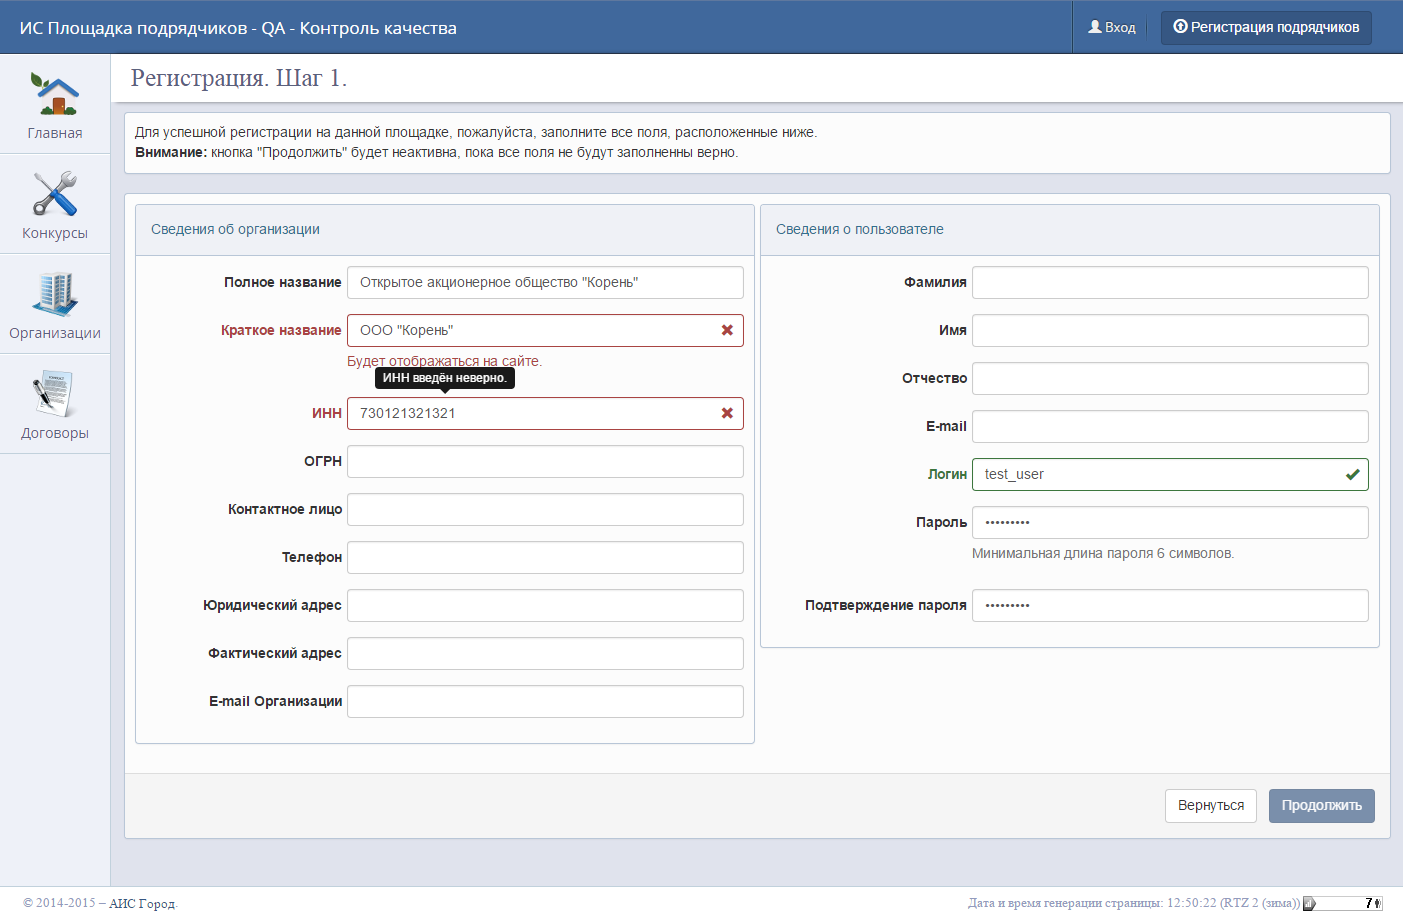
\includegraphics[width=\linewidth]{images/software-contractorRegistration.png}
			\caption{Страница заполнения основной информации при регистрации подрядчика}
			\label{img:software-contractorRegistration}
		\end{minipage}
		\hfill
	\end{center}
\end{figure}

После заполнения основной информации можно заполнить сведения о руководителе, членстве в СРО, заполнить графическое портфолио.

\paragraph{Подача заявки на одобрение РОКР}

Данное действие выполняется подрядной организацией.

Для того, чтобы подать заявку на одобрение подрядной организации региональным оператором капитального ремонта, следует зайти в личный кабинет (соответствующая ссылка в шапке сайта), перейти в меню второго уровня <<Заявки в РОКР>> и нажать на кнопку <<Подать заявку>>.
Схематично этот процесс показан на рисунке~\ref{img:software-contractorRequest}.

\begin{figure}[h!]
	\begin{center}
		\begin{minipage}[h]{\linewidth}
			\centering
			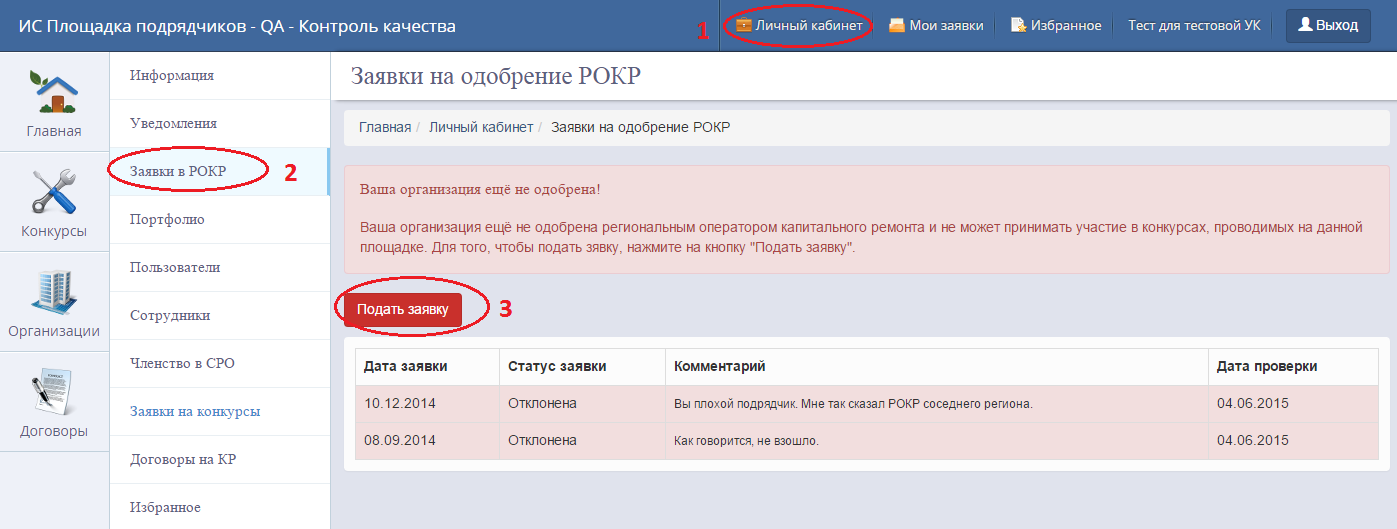
\includegraphics[width=\linewidth]{images/software-contractorRequest.png}
			\caption{Процесс подачи заявки на одобрение РОКР}
			\label{img:software-contractorRequest}
		\end{minipage}
		\hfill
	\end{center}
\end{figure}

\paragraph{Участие в розыгрыше}

Данное действие выполняется подрядной организацией.

Для того, чтобы принять участие в конкусе, необходимо получить одобрение от РОКР в участии на площадке.

Сперва следует зайти на страницу со списком конкурсов и выбрать необходимый конкурс со статусом <<Приём заявок>>.
Затем следует отобразить подробности конкурса, нажав на его названии.
Напротив необходимого лота есть кнопка со знаком <<+>>, либо же в подробностях лота есть кнопка <<Подать заявку>>.
При нажатии на одну из этих кнопок откроется страница подачи заявки на участие в розыгрыше права выпронять капитальный ремонт.
Примерное изображение страницы подачи заявки представлено на рисунке~\ref{img:software-contractorBid}.

\begin{figure}[h!]
	\begin{center}
		\begin{minipage}[h]{\linewidth}
			\centering
			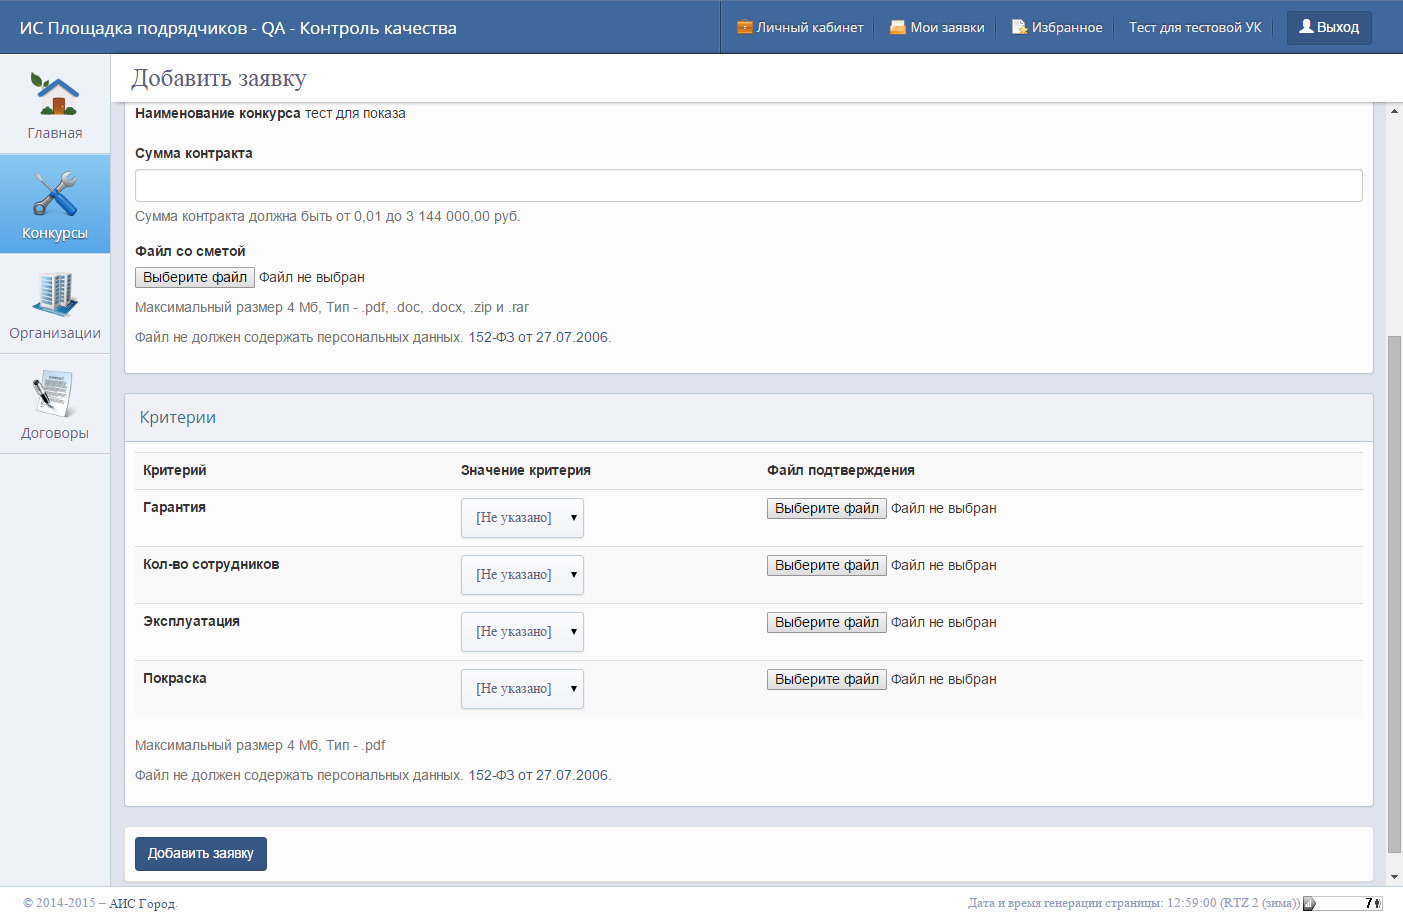
\includegraphics[width=\linewidth]{images/software-contractorBid.png}
			\caption{Страница подачи заявки на розыгрыш права проводить капитальный ремонт}
			\label{img:software-contractorBid}
		\end{minipage}
		\hfill
	\end{center}
\end{figure}

\paragraph{Одобрение подрядчика}

Данное действие выполняется региональным оператором капитального ремонта.

Для одобрения подрядной организации следует в меню <<Подрядчики>> перейти к странице <<Отбор подрядчиков>>.
На ней следует изменить необходимую заявку.
Для упрощения отображения можно использовать фильтр по статусу или организации.
На появившейся странице следует ввести статус заявки и комментарий, если она отклонена.
Изображение страницы изменения статуса заявки представлено на рисунке~\ref{img:software-hmRequest}.

\begin{figure}[h!]
	\begin{center}
		\begin{minipage}[h]{\linewidth}
			\centering
			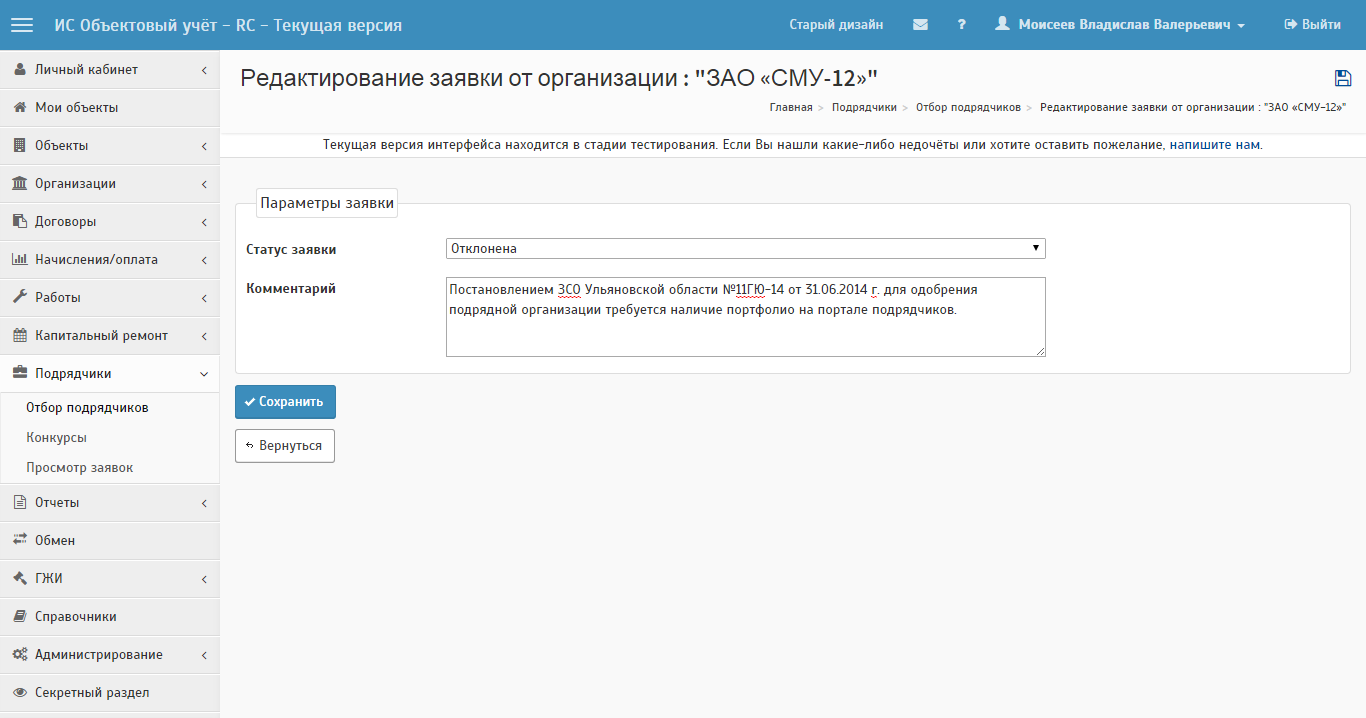
\includegraphics[width=\linewidth]{images/software-hmRequest.png}
			\caption{Страница одобрения заявки подрядчика}
			\label{img:software-hmRequest}
		\end{minipage}
		\hfill
	\end{center}
\end{figure}

Также при изменении заявки у подрядчика в личном кабинете появится уведомление об изменении статуса заявки на одобрение.
Пример уведомления об одобрении подрядчика показан на рисунке~\ref{img:software-contractorRequestNotify}.

\begin{figure}[h!]
	\begin{center}
		\begin{minipage}[h]{\linewidth}
			\centering
			
\includegraphics[width=\linewidth]{images/software-contractorRequestNotify.png}
			\caption{Уведомление об одобрении подрядчика}
			\label{img:software-contractorRequestNotify}
		\end{minipage}
		\hfill
	\end{center}
\end{figure}

\paragraph{Создание конкурса}

Данное действие выполняется региональным оператором капитального ремонта.

Для создания конкурса необходимо сперва создать запись о планах работ (сметах).
Следует зайти в меню <<Справочники>>, где в блоке <<Подрядчики>> перейти по ссылке <<Сметы>>.
После добавления необходимых данных откроется страница с подробностями информации о созданной смете.
На этой странице необходимо указать виды работ по смете.

После описания смет и видов работ по ним можно приступать к созданию конкурса.
Для этого в меню <<Подрядчики>> следует перейти на страницу <<Конкурсы>>.
После нажатия на кнопку <<Добавить конкурс>> откроется необходимая страница.
При верном вводе данных откроется страница подробностей конкурса, где можно создать необходимые лоты.
После создания лотов на странице их подробностей необходимо нажать на кнопку <<Прикрепить смету>> для добавления к лоту созданных ранее смет.

После прикрепления необходимых смет к лотам следует отобразить лоты и конкурсы на площадке подрядчиков.
Это можно сделать со страниц списка конкурсов (для конкурса) и подробностей конкурса (для лотов).

%\paragraph{Розыгрыш конкурса}
%Данное действие выполняется региональным оператором капитального ремонта.
%Для розыгрыша конкурса необходимо перейти на страницу подробностей конкурса.

\subsubsection{Исключительные ситуации и их обработка}

Система обрабатывает исключения трёх видов:

\begin{easylist}
& запрос пользователя ведёт на несуществующий маршрут приложения;
& запрос пользователя содержит данные, при которых возникла ошибка исполнения;
& запрос пользователя не проходит проверку веб-сервера (например, большой объём передаваемых данных или нарушение политики безопасности).
\end{easylist}

Для первого типа предусмотрена страница с текстом о том, что запрашиваемая страница не найдена.
На площадке подрядчиков вид такой страницы представлен на рисунке~\ref{img:software-contractorNotFound}.

\begin{figure}[h!]
	\begin{center}
		\begin{minipage}[h]{\linewidth}
			\centering
			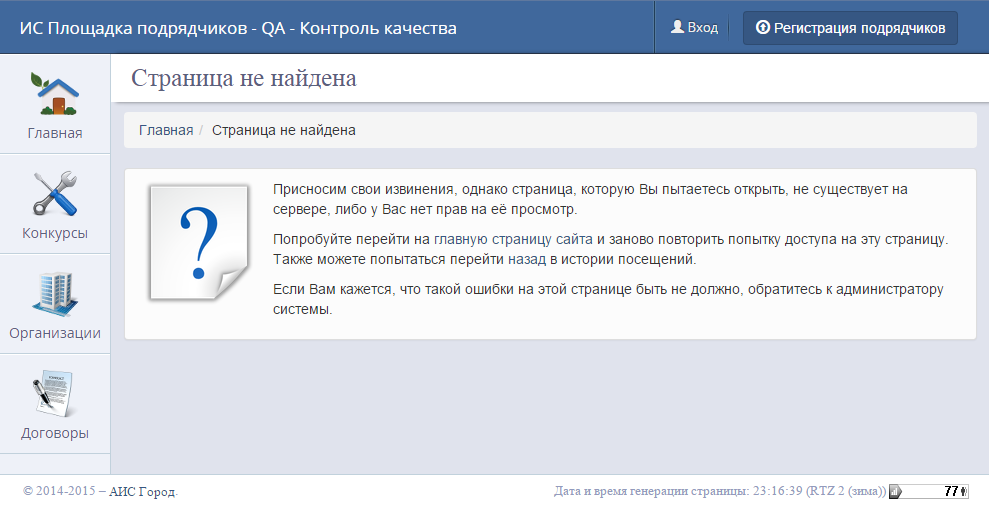
\includegraphics[width=\linewidth]{images/software-contractorNotFound.png}
			\caption{Страница при неправильной ссылке на площадке подрядчиков}
			\label{img:software-contractorNotFound}
		\end{minipage}
		\hfill
	\end{center}
\end{figure}

Второй и третий вид исключительных ситуаций могут либо выдавать блок с ошибкой в верхней части основной области страницы (как на рисунке~\ref{img:software-contractorErrorTop}) или отображать специальную страницу с ошибкой (как на рисунке~\ref{img:software-contractorErrorAll}).

\begin{figure}[h!]
	\begin{center}
		\begin{minipage}[h]{\linewidth}
			\centering
			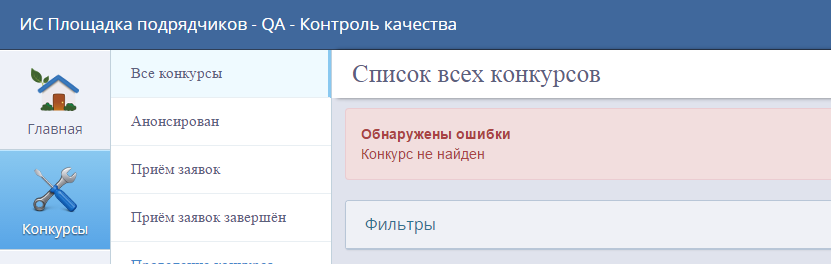
\includegraphics[width=\linewidth]{images/software-contractorErrorTop.png}
			\caption{Блок ошибки на площадке подрядчиков}
			\label{img:software-contractorErrorTop}
		\end{minipage}
		\hfill
	\end{center}
\end{figure}

\begin{figure}[h!]
	\begin{center}
		\begin{minipage}[h]{\linewidth}
			\centering
			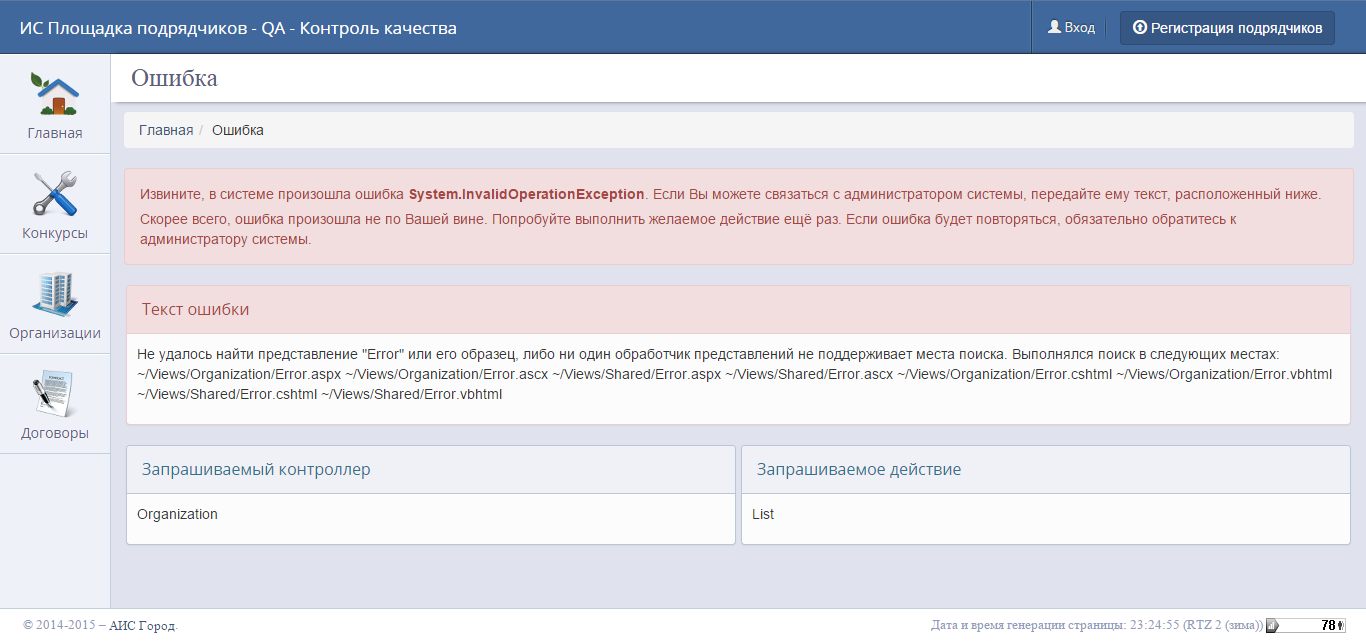
\includegraphics[width=\linewidth]{images/software-contractorErrorAll.png}
			\caption{Страница ошибки на площадке подрядчиков}
			\label{img:software-contractorErrorAll}
		\end{minipage}
		\hfill
	\end{center}
\end{figure}

\clearpage
\newpage